\let\negmedspace\undefined
\let\negthickspace\undefined
\documentclass[journal,12pt,onecolumn]{IEEEtran}
\usepackage{cite}
\usepackage{amsmath,amssymb,amsfonts,amsthm}
\usepackage{algorithmic}
\usepackage{graphicx}
\usepackage{textcomp}
\usepackage{xcolor}
\usepackage{txfonts}
\usepackage{listings}
\usepackage{enumitem}
\usepackage{mathtools}
\usepackage{gensymb}
\usepackage{comment}
\usepackage{caption}
\usepackage[breaklinks=true]{hyperref}
\usepackage{tkz-euclide} 
\usepackage{listings}

\usepackage{gvv}                                        
%\def\inputGnumericTable{}                                 
\usepackage[latin1]{inputenc}     
\usepackage{xparse}
\usepackage{color}                                            
\usepackage{array}                                            
\usepackage{longtable}                                       
\usepackage{calc}                                             
\usepackage{multirow}
\usepackage{multicol}
\usepackage{hhline}                                           
\usepackage{ifthen}                                           
\usepackage{lscape}
\usepackage{tabularx}
\usepackage{array}
\usepackage{float}
%\newtheorem{theorem}{Theorem}[section]
%\newtheorem{theorem}{Theorem}[section]
%\newtheorem{problem}{Problem}
%\newtheorem{proposition}{Proposition}[section]
%\newtheorem{lemma}{Lemma}[section]
%\newtheorem{corollary}[theorem]{Corollary}
%\newtheorem{example}{Example}[section]
%\newtheorem{definition}[problem]{Definition}

\begin{document}

\title{2.7.7}
\author{AI25BTECH11035 - SUJAL RAJANI}
% \maketitle
% \newpage
% \bigskip
%\begin{document}
{\let\newpage\relax\maketitle}
%\renewcommand{\thefigure}{\theenumi}
%\renewcommand{\thetable}{\theenumi}
% \newpage
% \bigskip
\textbf{QUESTION}
Construct a rectangle whose adjacent sides are of lengths 5cm and 3.5cm.
\textbf{SOLUTION}
 as  mentioned in question adjacent sides are of lengths 5cm and 3.5cm.
 \\
as nothing is mentioned in question about the points :
\\
so we are taking rectangle as ABCD :
\\
 where position vector of respective points are :
 \\
 \begin{align*}
     \vec{A}=\myvec{0\\0}, \vec{B}=\myvec{0\\5}, \vec{C}=\myvec{3\\5},\vec{D}=\myvec{3\\0},
 \end{align*}
 our assumed coordinates are satisfying all the properties of rectangle :
 \begin{align*}
     (\vec{B}-\vec{A})^\top(\vec{C}-\vec{B})=0
     \\
      (\vec{C}-\vec{B})^\top(\vec{D}-\vec{C})=0
      \\
       (\vec{D}-\vec{C})^\top(\vec{A}-\vec{D})=0
        \\
        (\vec{A}-\vec{D})^\top(\vec{B}-\vec{A})=0
 \end{align*}
 \begin{align*}
     (\vec{B}-\vec{A})^\top(\vec{B}-\vec{A})=25
     \\
     (\vec{C}-\vec{B})^\top(\vec{C}-\vec{B})=9
     \\
      (\vec{D}-\vec{C})^\top (\vec{D}-\vec{C})=25
      \\
      (\vec{A}-\vec{D})^\top(\vec{A}-\vec{D})=9
 \end{align*}
     

        \begin{figure}[H]
    \centering
    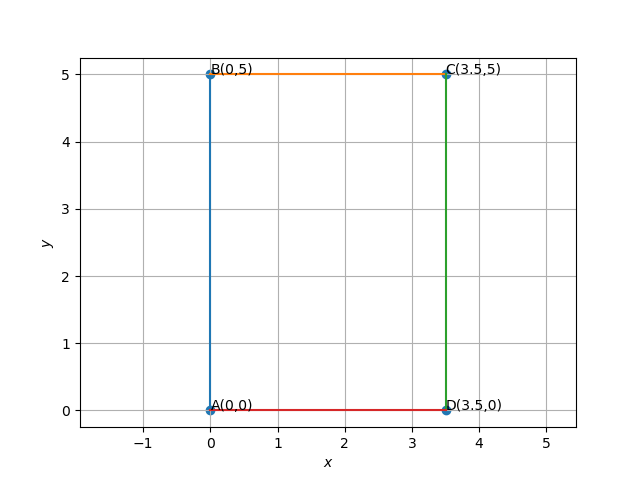
\includegraphics[width = 0.7\columnwidth]{figs/img.png}
    \caption*{}
    \label{figs}
\end{figure}

\end{document}